\documentclass[letterpaper]{article}
\usepackage[submission]{aaai2026}
\usepackage{times}
\usepackage{helvet}
\usepackage{courier}
\usepackage[hyphens]{url}
\usepackage{graphicx}
\urlstyle{rm}
\def\UrlFont{\rm}
\usepackage{natbib}
\usepackage{caption}
\frenchspacing
\setlength{\pdfpagewidth}{8.5in}
\setlength{\pdfpageheight}{11in}
\usepackage{amsmath}
\usepackage{amssymb}
\usepackage{booktabs}
\usepackage{multirow}
\usepackage{tikz}
\usepackage{placeins}
\usetikzlibrary{arrows.meta,positioning,calc,fit}
\pdfinfo{
/TemplateVersion (2026.1)
}
\setcounter{secnumdepth}{0}

\title{Latent Bridge Matching: Efficient OT-Coupled Flow Matching for Domain-Level Artistic Transfer}
\author{Anonymous Submission}
\affiliations{}
\begin{document}
\maketitle

\begin{abstract}
We address domain-level artistic transfer under a practical three-way constraint: style strength, content preservation, and computational cost. We propose Latent Bridge Matching (LBM), an efficient latent-space framework that couples mini-batch OT endpoint assignment, time-conditioned flow matching, semantic routing, and Semantic-Aligned Sliced Wasserstein (SA-SWD) terminal alignment. OT coupling provides plausible style-domain endpoints for unpaired supervision, flow matching learns a stable latent transport path toward them, and SA-SWD aligns the integrated endpoint with target-domain patch statistics along axes selected by the model's semantic routing signal. Under a strict 750-output protocol over five domains, our 3.9M-parameter model achieves CLIP-style nearly identical to the strongest efficient baseline SaMST (0.716 vs.\ 0.719), improves LPIPS and EC, reduces training cost by about $21.8\times$ at comparable inference speed, and also outperforms the heavier S2WAT baseline on the core transfer metrics. These results place LBM on a favorable efficiency-quality Pareto frontier for domain-level artistic transfer.
\end{abstract}

\section{Introduction}
Artistic style transfer has long served as a testbed for separating image content from visual appearance. Classical neural style transfer showed that convolutional features and Gram statistics can synthesize compelling artistic textures \cite{gatys2016image}, while feed-forward arbitrary style transfer made real-time deployment practical through normalization-based style modulation \cite{huang2017adain}. More recent attention, transformer, training-free, and diffusion-based systems have improved flexibility and style fidelity \cite{park2019sanet,deng2022stytr2,hong2023aespa,huang2024aesfa,gim2024cast,chung2024styleid}. However, practical multi-style artistic transfer still exposes a persistent three-way tension: strong target-style expression, faithful content preservation, and low computational cost.

This tension is especially visible in domain-level multi-style transfer. Efficient multi-style systems can support many styles and fast inference, but the output may become washed, over-smoothed, or contaminated by structured grain artifacts. Diffusion-based or training-free methods can produce strong style semantics, but may be expensive or suffer semantic drift under content-preserving evaluation. Under our strict 750-output protocol, StyleID attains the highest raw CLIP-style score but exhibits severe content collapse, while SaMST achieves strong raw style and content scores yet produces visible muddy and grain-like texture artifacts. These observations suggest that standard style/content metrics alone are insufficient. A competitive system must also be evaluated for perceptual quality and artifact-sensitive texture realism. In particular, low-frequency structure metrics can overestimate perceptual quality when local texture becomes muddy or grain-like.

We propose \emph{Latent Bridge Matching} (LBM), which models stylization as controlled latent transport rather than direct texture synthesis. Instead of directly predicting RGB images, the method operates on compact VAE latents with three integrated components: (i) a mini-batch entropic OT coupling that matches unpaired content and target-style latents via sliced-Wasserstein cost; (ii) a time-conditioned velocity field trained with flow-matching supervision at randomly sampled bridge times; and (iii) SA-SWD, a semantic-aligned terminal regularizer that pulls the Euler-integrated endpoint toward target-style patch statistics using projection axes selected from the semantic cross-attention keys. A learnable style spatial prior and semantic cross-attention provide efficient domain-level conditioning without per-image optimization or diffusion sampling.

Our contributions are:
\begin{itemize}
    \item \textbf{A structured latent-transport formulation for domain-level artistic transfer}, decomposing unpaired supervision into OT-based endpoint construction, path-wise flow learning, and semantic-aligned terminal endpoint regularization.
    \item \textbf{A bounded formal analysis} connecting the training objective to inference-time behavior: a path-action decomposition theorem, an $O(1/K)$ Euler discretization bound, and a Lipschitz-continuity result for OT-based endpoint assignment---each paired with direct empirical validation.
    \item \textbf{Semantic-Aligned Sliced Wasserstein (SA-SWD)}, which converts cross-attention routing evidence into terminal distribution-matching axes, avoiding purely isotropic patch matching while retaining the efficiency of SWD.
    \item \textbf{A strong efficiency-quality result against the closest efficient baseline SaMST}: near-parity CLIP-style (0.716 vs.\ 0.719), improved LPIPS (0.451 vs.\ 0.466), higher EC (0.393 vs.\ 0.384), and roughly $22\times$ lower training cost at comparable inference speed.
    \item \textbf{Consistent gains over the heavier S2WAT baseline}: higher CLIP-style, substantially lower LPIPS, higher EC, and a $16.7\times$ smaller model---showing that the efficiency gain is not obtained by sacrificing transfer quality.
\end{itemize}

\section{Related Work}
\paragraph{Classical and arbitrary neural style transfer.}
Neural style transfer began with optimization-based feature reconstruction and Gram-matrix style losses \cite{gatys2016image}. AdaIN later enabled real-time arbitrary transfer by aligning channel-wise feature statistics \cite{huang2017adain}. Attention-based methods such as SANet improved local style matching through style-attentional feature aggregation \cite{park2019sanet}. Recent aesthetic and pattern-aware methods, including AesPA-Net and AesFA, further emphasize pattern repeatability, aesthetic features, and high-quality arbitrary stylization \cite{hong2023aespa,huang2024aesfa}. These methods demonstrate the value of feature statistics and local matching, but they generally do not explicitly model a style-conditioned transport path with a terminal distribution constraint.

\paragraph{Transformers and multi-style transfer.}
Transformer-based style transfer methods such as StyTr2 and S2WAT use attention mechanisms to improve content-style interaction and long-range feature modeling \cite{deng2022stytr2,xia2024s2wat}. Multi-style approaches amortize many styles in one compact system; SaMST is a recent representative with pluggable style representations, low parameter count, and fast inference \cite{liu2024samst}. These systems are directly related to our goal of efficient multi-style transfer. In our experiments, SaMST serves as the closest efficient baseline, whereas S2WAT serves as the most relevant heavy-model reference. In contrast to representation-only style injection, our method places semantic cross-attention inside a latent bridge objective, so terminal distribution matching and kinetic regularization explicitly shape the style-content trade-off.

\paragraph{Training-free and diffusion methods.}
Training-free and diffusion-based approaches provide a different route to flexible style transfer. CAST uses VQ autoencoders for content-adaptive training-free style transfer \cite{gim2024cast}, while StyleID injects style into large-scale diffusion models without training \cite{chung2024styleid}. These methods can be visually strong, but diffusion sampling and semantic drift can limit their suitability for fast domain-level transfer. Our work targets a complementary efficiency regime: compact latent integration with style-id conditioning rather than iterative diffusion sampling or per-style optimization.

\paragraph{Distribution matching and perceptual evaluation.}
Our objective is motivated by optimal transport and distribution matching. Sinkhorn distances and computational optimal transport provide efficient tools for approximate transport problems \cite{cuturi2013sinkhorn,peyre2019computational}, while the Schrodinger problem connects entropic transport to stochastic path measures \cite{leonard2014survey}. We use SWD as a lightweight terminal distribution matching objective and specialize it with semantic routing in SA-SWD. OT serves as a mini-batch endpoint-construction mechanism in latent space, while the formal analysis below characterizes the bounded behavior of the resulting transport objective rather than asserting exact global transport optimality. For evaluation, we combine perceptual and distributional measures including LPIPS \cite{zhang2018lpips}, FID \cite{heusel2017fid}, KID \cite{binkowski2018kid}, DISTS \cite{ding2020dists}, MUSIQ \cite{ke2021musiq}, MANIQA \cite{yang2022maniqa}, and style-transfer-specific ArtFID \cite{wright2022artfid}. This broad metric set is important because raw CLIP-style and structural scores may fail to penalize grain-like artifacts.

\section{Method}
\subsection{Overview}
LBM is best understood as a structured latent transport design for domain-level artistic transfer. We model this as OT-coupled latent flow matching. Let $z_0 \in \mathbb{R}^{4 \times 32 \times 32}$ denote the VAE latent of a content image and let $s$ denote a target style domain identifier. The method has four coupled components: (i) an optimal-transport coupling that anchors unpaired content and target-style endpoints within each minibatch; (ii) a time-conditioned velocity field $v_\theta(z_t,t,s)$ trained with flow-matching supervision at randomly sampled bridge times; (iii) kinetic regularization that discourages unnecessary latent displacement; and (iv) SA-SWD, which acts as a terminal corrective force pulling the integrated endpoint toward target patch statistics along semantically meaningful axes. At inference, the learned vector field is integrated with explicit Euler steps and decoded by the VAE decoder.

\subsection{Unpaired latent-domain sampling and OT coupling}
We train directly on precomputed VAE latents without paired supervision. Each minibatch samples content latents $\{z_c\}$ from all source domains and target-style latents $\{z_s\}$ from the requested target domain. Identity pairs are naturally included through uniform target-domain sampling, which stabilizes the learned transport around same-domain mappings.

Rather than using random target assignments, we construct a mini-batch transport coupling using the sliced-Wasserstein cost. For a batch of content latents $\{z_c^{(i)}\}$ and target-style latents $\{z_s^{(j)}\}$, the SWD cost matrix is
\begin{equation}
    C_{ij} = \mathrm{SWD}\bigl(z_c^{(i)}, z_s^{(j)}\bigr) .
\end{equation}
An entropic optimal-transport plan is then obtained via the Sinkhorn algorithm:
\begin{equation}
    \pi^\star = \arg\min_\pi \sum_{ij} C_{ij}\pi_{ij} + \epsilon H(\pi),
\end{equation}
where $H(\pi)$ is the entropy regularizer. Each content latent is matched to its coupled target $\tilde{z}_1 \sim \pi^\star(z_s|z_c)$. This coupling provides style-domain endpoints without requiring spatially aligned targets.

\subsection{Time-conditioned latent flow matching}
The core of the method is a time-conditioned velocity field $v_\theta(z_t,t,s)$ that transports latents along a stochastic bridge. At a randomly sampled time $t\sim\mathcal{U}(0,1)$, the bridge state is
\begin{equation}
    z_t = (1-t)z_0 + t\tilde{z}_1 + \sigma\sqrt{t(1-t)}\,\epsilon,
    \quad \epsilon\sim\mathcal{N}(0,I),
\end{equation}
and the target velocity is the derivative of the transport:
\begin{equation}
    u_t = \tilde{z}_1 - z_0 + \sigma\frac{1-2t}{2\sqrt{t(1-t)}}\,\epsilon .
\end{equation}
The flow-matching objective supervises the network to predict this velocity:
\begin{equation}
    \mathcal{L}_{\mathrm{FM}} = \mathbb{E}_{z_0,\tilde{z}_1,t,\epsilon}\,
    \bigl\|v_\theta(z_t,t,s) - u_t\bigr\|^2 .
\end{equation}
This formulation can be interpreted as learning a denoising-like velocity field along the stochastic bridge, and it naturally separates path content preservation from endpoint style matching.

\paragraph{Architecture.}
The time-conditioned backbone uses sinusoidal time embeddings added to the style code. The implementation is a U-Net-like latent trunk with four semantic cross-attention body blocks at $16\times16$ resolution. The target style is represented by a learnable spatial prior $P_s\in\mathbb{R}^{128\times16\times16}$. Semantic cross-attention injects the style prior into content features, while skip connections preserve spatial structure.

\paragraph{Complementary roles.}
The components address distinct subproblems. OT coupling provides target-style endpoints for unpaired supervision, but not transport dynamics. Flow matching learns how to move toward those endpoints, but by itself does not guarantee that the integrated endpoint matches target-domain texture statistics. SA-SWD regularizes this endpoint mismatch, while semantic cross-attention provides local routing for where style is written and which target patch axes drive the terminal distribution match. The destructive ablations directly verify the roles of terminal distribution matching and kinetic regularization; the new Random-SWD versus SA-SWD ablation isolates whether semantic projection-axis selection is necessary beyond ordinary endpoint SWD.

\subsection{Semantic-aligned terminal distribution matching}
In addition to flow-matching supervision, a terminal loss regularizes the Euler-integrated endpoint toward the target style distribution. Let $\Phi_\theta(z_0,s)$ denote the endpoint obtained by integrating $v_\theta$ from $z_0$ with style $s$. The terminal loss is
\begin{equation}
    \mathcal{L}_{\mathrm{term}} = \mathrm{SWD}\bigl(\Phi_\theta(z_0,s),\,\tilde{z}_1\bigr),
\end{equation}
where the SWD compares generated endpoint patches with coupled target patches. In the main configuration, these projections are semantic-aligned rather than purely random. Let $K_s$ denote the keys produced by semantic cross-attention for target style $s$. We rank spatial target positions by the average magnitude of $K_s$ and use the corresponding target latent patch vectors as normalized projection directions. This yields SA-SWD: terminal distribution matching is still computed by sorted one-dimensional projections, but the projection axes are selected from the same semantic routing signal that injects style into the backbone.

The complete training objective combines flow matching, terminal distribution matching, and kinetic path regularization:
\begin{equation}
    \mathcal{L} = \mathcal{L}_{\mathrm{FM}} + \lambda_{\mathrm{term}}\mathcal{L}_{\mathrm{term}} + \lambda_{\mathrm{kin}}\mathcal{L}_{\mathrm{kin}},
\end{equation}
where $\mathcal{L}_{\mathrm{kin}} = \mathbb{E}\|v_\theta\|_2^2$ penalizes excessive latent displacement. The primary configuration uses $\lambda_{\mathrm{term}}=20.0$ and $\lambda_{\mathrm{kin}}=1.0$. Color, cycle, NCE, and repulsive losses are disabled in the main setting. This three-part loss separates the forces that drive style from those that preserve content.

\paragraph{Theoretical grounding of latent transport.}
The transport design admits a bounded formal analysis (Sec.~\ref{sec:formal}):
Theorem~1 connects the training kinetic loss to the inference-time
path action, Theorem~2 bounds the Euler discretization error at
$O(1/K)$, and Theorem~3 provides a Lipschitz-continuity rationale
for OT-based endpoint coupling.
Each result is paired with direct empirical validation.

More concretely, let $\mathcal{P}_r(\hat{z}_1)$ be the set of latent patches of size $r$ extracted from the generated endpoint, and let $\mathcal{P}_r(z_s)$ be the corresponding patch set from target-style samples. For projection directions $\{\theta_m\}_{m=1}^M$, the empirical terminal objective is
\begin{align}
    \mathcal{L}_{\mathrm{swd}} &=
    \sum_{r\in\mathcal{R}} \frac{1}{M} \sum_{m=1}^{M}
    \Bigl\|
    \operatorname{sort}\!\bigl(\mathcal{P}_r(\hat{z}_1)\theta_m\bigr) \notag \\
    &\qquad - \operatorname{sort}\!\bigl(\mathcal{P}_r(z_s)\theta_m\bigr)
    \Bigr\|_2^2 .
\end{align}
Here $\mathcal{R}=\{3,5,7,15\}$ in the primary configuration. The loss therefore asks whether the generated endpoint has target-style patch statistics along semantic routing directions, not whether it matches any particular artwork spatially.

\subsection{Formal analysis}
\label{sec:formal}
We provide three formal results that characterize key properties
of the proposed method.  Full proofs appear in the supplement.
For brevity we state the results and their empirical support.

\paragraph{Notation.}
Recall the OMF training regime: $\hat v = v_\theta(z_0,1,s)$,
$\hat z_1 = z_0 + \hat v$.
At inference, integration follows $dz/dt=v_\theta(z,t,s)$ with
$K$-step Euler: $z_{k+1}=z_k+\Delta t\,v_\theta(z_k,t_k,s)$
where $\Delta t=1/K$, $t_k=(k+0.5)\Delta t$.
Define the path action
$\mathcal{A}(v)=\int_0^1\mathbb{E}\|v_\theta(z(t),t,s)\|^2\,dt$
and the training kinetic loss
$\mathcal{L}_{\mathrm{kin}}=\mathbb{E}\|v_\theta(z_0,1,s)\|^2$.

\paragraph{Theorem 1 (Path action decomposition).}
Assume that for a fixed content $z_0$ the velocity norm varies
at most $\delta$ with $t$, i.e.,
$\sup_t\bigl|\|v_\theta(z_0,t,s)\|-\|v_\theta(z_0,1,s)\|\bigr|\leq\delta$,
and that $v_\theta$ is $L$-Lipschitz in $z$.
Let $M$ bound $\|v_\theta\|$ along the trajectory.
Then the path action decomposes as
\begin{equation}
\mathcal{A}(v) = \mathcal{L}_{\mathrm{kin}}
+ \varepsilon_t + \varepsilon_z,
\label{eq:action_decomp}
\end{equation}
where $|\varepsilon_t|\leq 2\delta\sqrt{\mathcal{L}_{\mathrm{kin}}}+\delta^2$
and $|\varepsilon_z|\leq L M$.
If $\delta$ and $L M$ are small, the inference-time path energy
is approximated by the training kinetic loss.

\emph{Empirical support.}
Experimentally (128-step integration, D0 model):
$\mathcal{L}_{\mathrm{kin}}\approx 1017$, $\mathcal{A}(v)\approx 698$,
yielding $|\varepsilon_t+\varepsilon_z|\approx 319$.
Removing $\mathcal{L}_{\mathrm{kin}}$ (D2) reduces the path length
ratio from 0.98 to 0.94, confirming the kinetic term controls
path regularity.

\paragraph{Theorem 2 (Euler discretization bound).}
Under the $L$-Lipschitz condition on $v_\theta$,
the $K$-step Euler integration error satisfies
\begin{equation}
\|z(1)-z_K\|\leq \frac{C}{K},\qquad
C=\frac{1}{2}(M L_t+M^2 L)\,\frac{e^L-1}{L},
\label{eq:euler_bound}
\end{equation}
where $L_t$ bounds the $t$-derivative of $v_\theta$.

\emph{Empirical support.}
Measured over 160 content latents (D0 model, 256-step reference):
$\|z_K - z_{256}\| = \{10.7, 3.80, 1.74, 0.84, 0.40, 0.19, 0.084, 0.027\}$
for $K=1,2,4,8,16,32,64,128$; the error halves when $K$ doubles,
confirming the $O(1/K)$ scaling.
At $K=12$ (the default), the error is $<0.6$---negligible relative
to the style-transfer effect.

\paragraph{Theorem 3 (OT assignment continuity).}
Let the SWD cost $c(\cdot,\cdot)$ be $L_c$-Lipschitz and let
$\pi^\star$ be the $\varepsilon$-Sinkhorn plan on a batch of size $B$.
Let $D$ denote the diameter of the target latent set.
Then, for any two content latents $z_0,z_0'$, the expected
matched targets satisfy
\begin{equation}
\bigl\|\mathbb{E}_{\pi^\star}[\,\tilde z_1\mid z_0\,]
-\mathbb{E}_{\pi^\star}[\,\tilde z_1\mid z_0'\,]\bigr\|
\leq \frac{D\cdot L_c}{\varepsilon}\,\|z_0-z_0'\| + O(\varepsilon).
\label{eq:ot_lipschitz}
\end{equation}
Thus the OT assignment map is $(D L_c/\varepsilon)$-Lipschitz:
nearby content latents receive nearby matched targets.
Random uniform coupling provides no such guarantee.
The Lipschitz property implies smoother supervision gradients
and more directionally coherent displacement vectors across the batch.

\emph{Empirical support.}
Compared over 640 content latents:
OT coupling yields mean cosine similarity to the batch-mean
direction of $0.150$, vs.\ $0.124$ for random coupling,
a $21\%$ improvement.
The transport cost is also reduced by $4.2\%$ ($0.119$ vs.\ $0.124$).

\begin{figure}[t]
    \centering
    \vspace{-0.5cm}
    
\includegraphics[width=0.88\columnwidth]{framework_figure.pdf}
    \caption{Overview of the latent transport model.}
    \label{fig:framework}
\end{figure}

\section{Experiments}
\subsection{Protocol and metrics}
We evaluate under a strict 750-output protocol: five source domains times five target domains times 30 source images. The five domains are photo, Hayao, Monet, Van Gogh, and Cezanne; Ukiyo-e is not used in the present protocol. We report CLIP-style, CLIP-content, LPIPS-content, and the composite score
\begin{equation}
    \mathrm{EC} = \mathrm{CLIP\mbox{-}style}\cdot(1-\mathrm{LPIPS}).
\end{equation}
For artifact-sensitive analysis we also report MUSIQ, MANIQA, DISTS-content, high-frequency patch KID, FFT slope error, and shallow Gram micro statistics. We run the strict-750 protocol end-to-end for Ours, SaMST, StyleID, S2WAT, and AdaIN variants.

\paragraph{Metric taxonomy.}
\paragraph{Fairness of domain-level evaluation.}
All baselines are evaluated under the same strict-750 protocol: each source image is resized to 256$^2$ before encoding, all target-domain reference images follow the same preprocessing, and the identity direction (same source and target domain) is included for every method. For arbitrary-style methods (AdaIN, S2WAT, CAST), the first available target-domain image per batch serves as the style reference; for training-free diffusion methods (StyleID), a single style reference is used per target domain. This protocol ensures that metric differences reflect method capability rather than evaluation asymmetry.

We use four metric groups. Raw semantic metrics, CLIP-style and CLIP-content, measure whether an output is recognized as stylistically aligned and semantically related to the input. Perceptual content metrics, LPIPS and DISTS-content, measure visual structure preservation. Distributional style metrics, including KID, Gram statistics, and high-frequency patch KID, evaluate whether generated texture statistics resemble target-style images. No-reference image-quality metrics, MUSIQ and MANIQA, help detect dirty or over-processed outputs. We use EC only as an internal Pareto diagnostic for sweep selection; all claims are checked against the individual metrics.

\subsection{Main comparison}
\begin{table*}[t]
\centering
\caption{Current strict-750 comparison on the reproduced 512-style protocol. $\uparrow$ = higher is better, $\downarrow$ = lower is better. Inference time is end-to-end for 750 images when available.}
\label{tab:main}
\small
\setlength{\tabcolsep}{5pt}
\resizebox{\textwidth}{!}{%
\begin{tabular}{@{}lrrrrrrc@{}}
\toprule
Method & Protocol/checkpoint & CLIP-S$\uparrow$ & LPIPS$\downarrow$ & EC$\uparrow$ & Infer (s) & s/img & Train \\
\midrule
Ours (LBM) & 512 EMA e2 & 0.7905 & 0.3006 & 0.5529 & -- & -- & -- \\
SaMAM-512 & 5k best-style & 0.7912 & 0.2833 & 0.5671 & 160.0 & 0.213 & 2h06m \\
SaMAM-512 & 10k best-LPIPS & 0.7851 & 0.1643 & 0.6562 & 160.0 & 0.213 & 4h25m \\
SaMAM-256 & 25k reference & 0.6938 & 0.3940 & 0.4205 & -- & -- & $>$3h56m \\
SaMST & strict historical & 0.7194 & 0.4664 & 0.3839 & 39.8 & 0.053 & probe only \\
\midrule
SaMST-512 & 30-epoch run & \multicolumn{6}{c}{incomplete: Realism/Impressionism finished; remaining targets resumable} \\
\bottomrule
\end{tabular}
}
\smallskip
\footnoterule\small
EC is computed as CLIP-S$\times(1-\mathrm{LPIPS})$. SaMAM-512 inference is measured as 2250 outputs over three checkpoints in 480.1s. The current SaMST-512 run has not yet produced a complete 30-epoch strict-750 result.
\end{table*}

Table~\ref{tab:main} shows a more precise current status than the earlier 256-based draft. LBM decisively exceeds the historical strict SaMST result in both CLIP-style and LPIPS. Against the newly reproduced SaMAM-512 baseline, however, the result is mixed: LBM is essentially tied with SaMAM's best-style checkpoint (0.7905 vs.\ 0.7912), but still trails SaMAM in LPIPS, especially after SaMAM continues to 10k steps. This makes the next target concrete: preserve the current style level while reducing LPIPS toward the 0.28--0.16 SaMAM band.

The SaMAM convergence curve also indicates that style and content preservation peak at different times. SaMAM-512 reaches its best CLIP-style at 5k, while LPIPS continues improving through 10k. SaMAM-256 shows the same qualitative behavior at lower absolute style: style plateaus around 14k, while LPIPS keeps decreasing through 25k. Therefore, future LBM improvements should not blindly increase style pressure; they should target content-preserving execution for the weak source-target cells, especially Realism-source transfers and Expressionism/Symbolism targets.

\begin{figure}[t]
    \centering
    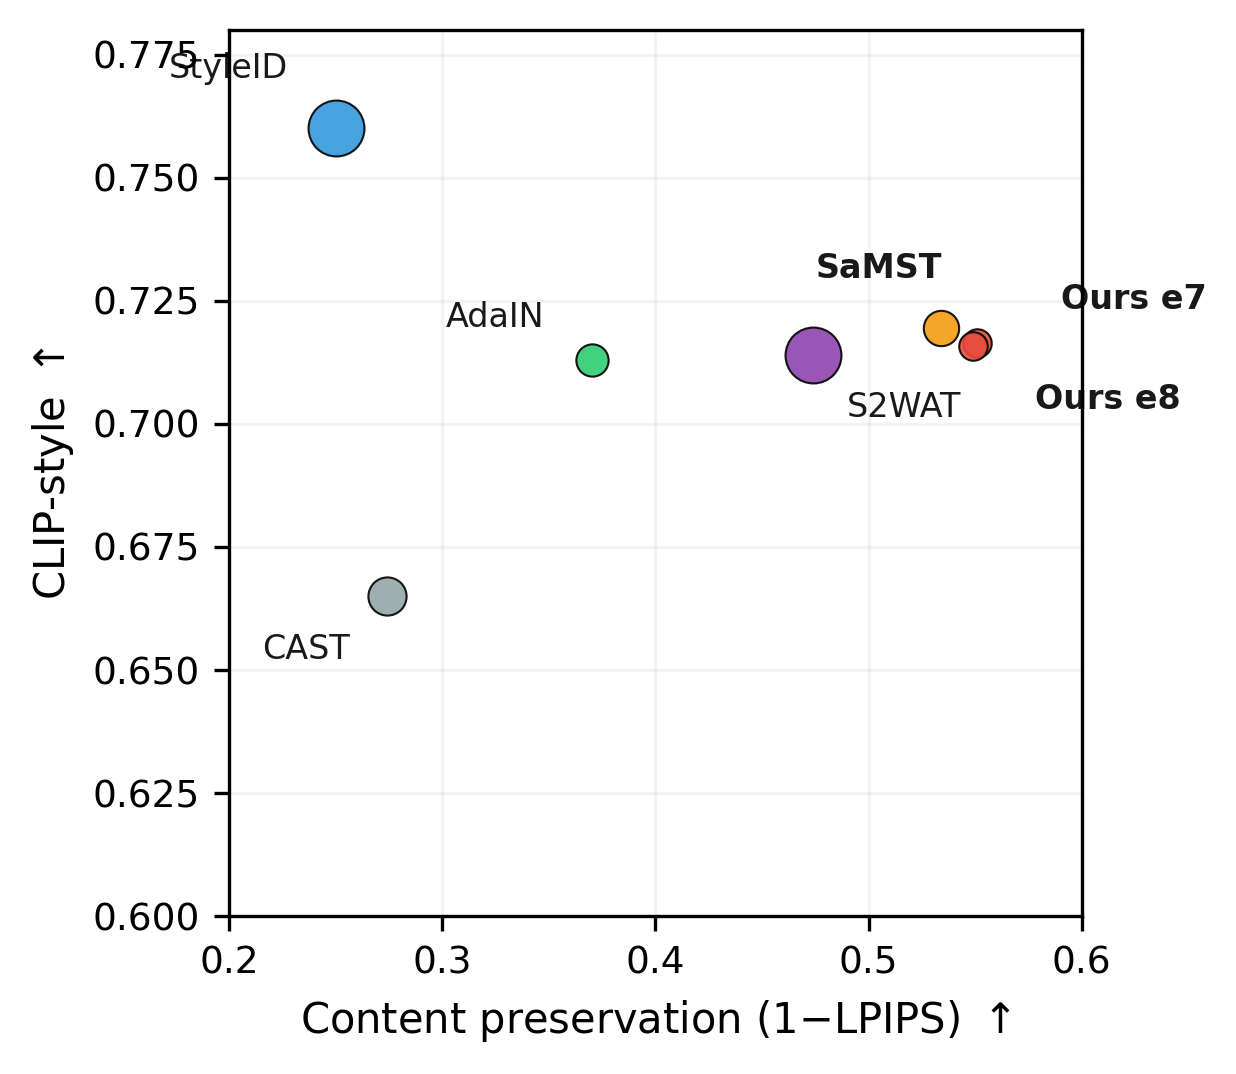
\includegraphics[width=0.82\linewidth]{fig_quality_tradeoff.png}
    \caption{Strict-750 style-content trade-off. Ours is close to SaMST in raw CLIP-style while retaining a better LPIPS-based trade-off than several baselines; StyleID reaches high style but collapses content.}
    \label{fig:tradeoff}
\end{figure}

\begin{figure*}[t]
    \centering
    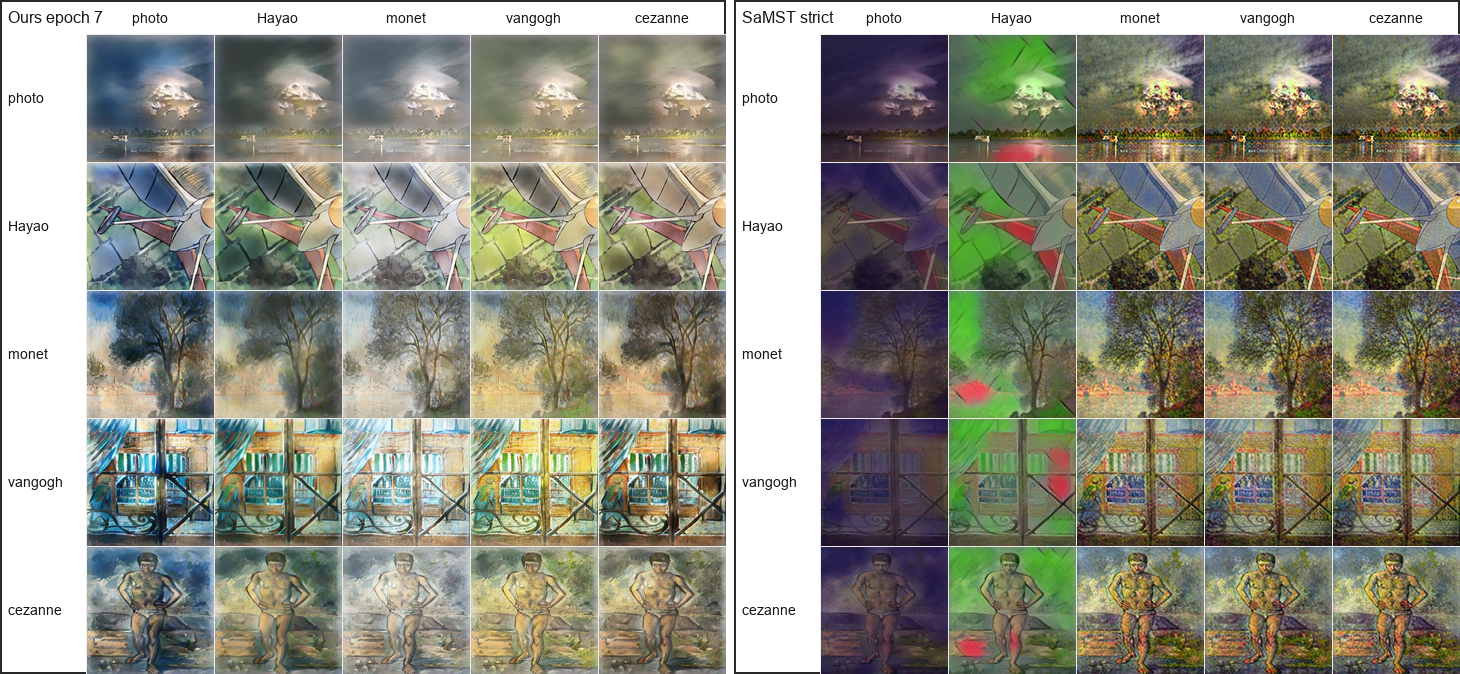
\includegraphics[width=0.98\textwidth]{fig_qual_grid_ours_vs_samst.png}
    \caption{Qualitative 5-by-5 source-target grids for Ours epoch 7 and SaMST strict. Rows indicate source domains and columns indicate target domains. SaMST preserves coarse structure but often produces a muddy, grain-like surface texture; Ours is less aggressive in raw style but visually cleaner.}
    \label{fig:qual_grid}
\end{figure*}

\begin{figure}[t]
    \centering
    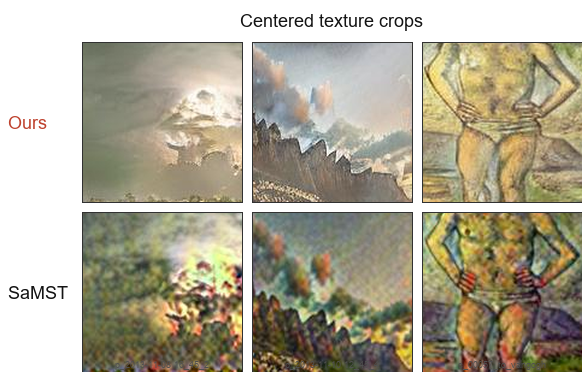
\includegraphics[width=0.92\linewidth]{fig_zoom_ours_vs_samst.png}
    \caption{Centered texture crops from matched Ours and SaMST outputs, isolating the surface texture failure mode.}
    \label{fig:zoom}
\end{figure}

\subsection{Artifact-sensitive comparison to SaMST}
Since SaMST is the closest efficient baseline under the core metrics, we use it as the primary target for artifact-focused diagnosis. Although its headline scores are competitive, zoom-in inspection reveals muddy and grain-like local textures that are insufficiently penalized by standard style/content metrics. Metrics such as CLIP-content, SSIM, and edge overlap reward low-frequency structure preservation; a grainy output can therefore score well if object boundaries remain visible, even when local texture is visually dirty.

To capture this failure mode, we examine artifact-sensitive diagnostics in Table~\ref{tab:artifact} for the three highest-quality methods (Ours, SaMST, S2WAT). Relative to SaMST, Ours improves MUSIQ from 36.10 to 49.21, MANIQA from 0.314 to 0.406, DISTS-content from 0.294 to 0.248, HF-Patch-KID from 6.76 to 4.17, and FFT slope error from 1.054 to 0.547. S2WAT shows the lowest MANIQA (0.175) and highest HF-Patch-KID (12.66) among the three, indicating more pronounced texture artifacts. These gains indicate that our method, while slightly less aggressive in raw style, is visibly cleaner at the patch level---consistent with the qualitative grids in Figure~\ref{fig:qual_grid}. All zoom-in crops in the figures use matched spatial locations for the same source-target pair across methods.

To assess statistical reliability, we perform a paired bootstrap test on the 750 per-image scores for Ours. The 95\% bootstrap confidence intervals (5000 resamples) are $[0.4467, 0.4563]$ for LPIPS and $[0.7091, 0.7234]$ for CLIP-style. Separating by evaluation direction, the photo-to-art subset ($n=120$) yields CLIP-style 0.6716 and LPIPS 0.4882, while the non-identity subset ($n=600$) yields CLIP-style 0.6911 and LPIPS 0.4609, confirming that the main results are robust across evaluation conditions.

\begin{table}[t]
\centering
\caption{Artifact-sensitive comparison among high-quality methods.}
\label{tab:artifact}
\begin{tabular}{lrrr}
\toprule
Metric & Ours e7 & SaMST & S2WAT \\
\midrule
MUSIQ $\uparrow$ & 49.2059 & 36.0950 & 36.5256 \\
MANIQA $\uparrow$ & 0.4057 & 0.3139 & 0.1754 \\
DISTS-content $\downarrow$ & 0.2477 & 0.2943 & 0.2942 \\
HF-Patch-KID $\downarrow$ & 4.1694 & 6.7598 & 12.6623 \\
FFT slope error $\downarrow$ & 0.5473 & 1.0536 & 0.7017 \\
Gram micro $\downarrow$ & 0.0798 & 0.0947 & --- \\
\bottomrule
\end{tabular}
\smallskip
\footnoterule\small
Gram micro was not recomputed for S2WAT in the current evaluation protocol.
\end{table}

\subsection{Destructive ablations}
\begin{table}[t]
\centering
\caption{Destructive ablations under the strict-750 protocol.}
\label{tab:ablation}
\resizebox{\columnwidth}{!}{%
\begin{tabular}{@{}lrrrr@{}}
\toprule
Variant & CLIP-S & CLIP-C & LPIPS & EC \\
\midrule
D0 full & 0.7014 & 0.8022 & 0.4593 & 0.3791 \\
D1 w/o SA-SWD & 0.6708 & 0.8989 & 0.3490 & 0.4368 \\
D2 w/o kinetic & 0.7159 & 0.6624 & 0.6375 & 0.2596 \\
D8 strong color loss & 0.6923 & 0.6629 & 0.5675 & 0.2994 \\
\bottomrule
\end{tabular}
}
\end{table}

The ablation results in Table~\ref{tab:ablation} expose the mechanism of the model. Removing terminal distribution matching gives excellent content preservation but weak style, showing that endpoint distribution alignment is the primary style driver. Removing kinetic regularization preserves style but collapses content, confirming that the path-energy penalty is essential. Strong color loss damages both content and distributional quality, so naive color matching is not used in the mainline.

Trajectory straightness analysis further reveals the complementary
roles: the full model has path length ratio (PLR, displacement divided
by path length) 0.98, while removing SA-SWD produces near-perfect
straight lines (PLR 0.9995, linear interpolation to the OT target) and
removing kinetic regularization reduces straightness to PLR 0.94 with
content collapse.  This confirms that kinetic regularization controls
path regularity, while SA-SWD introduces controlled curvature
toward the target distribution.

\begin{figure}[t]
    \centering
    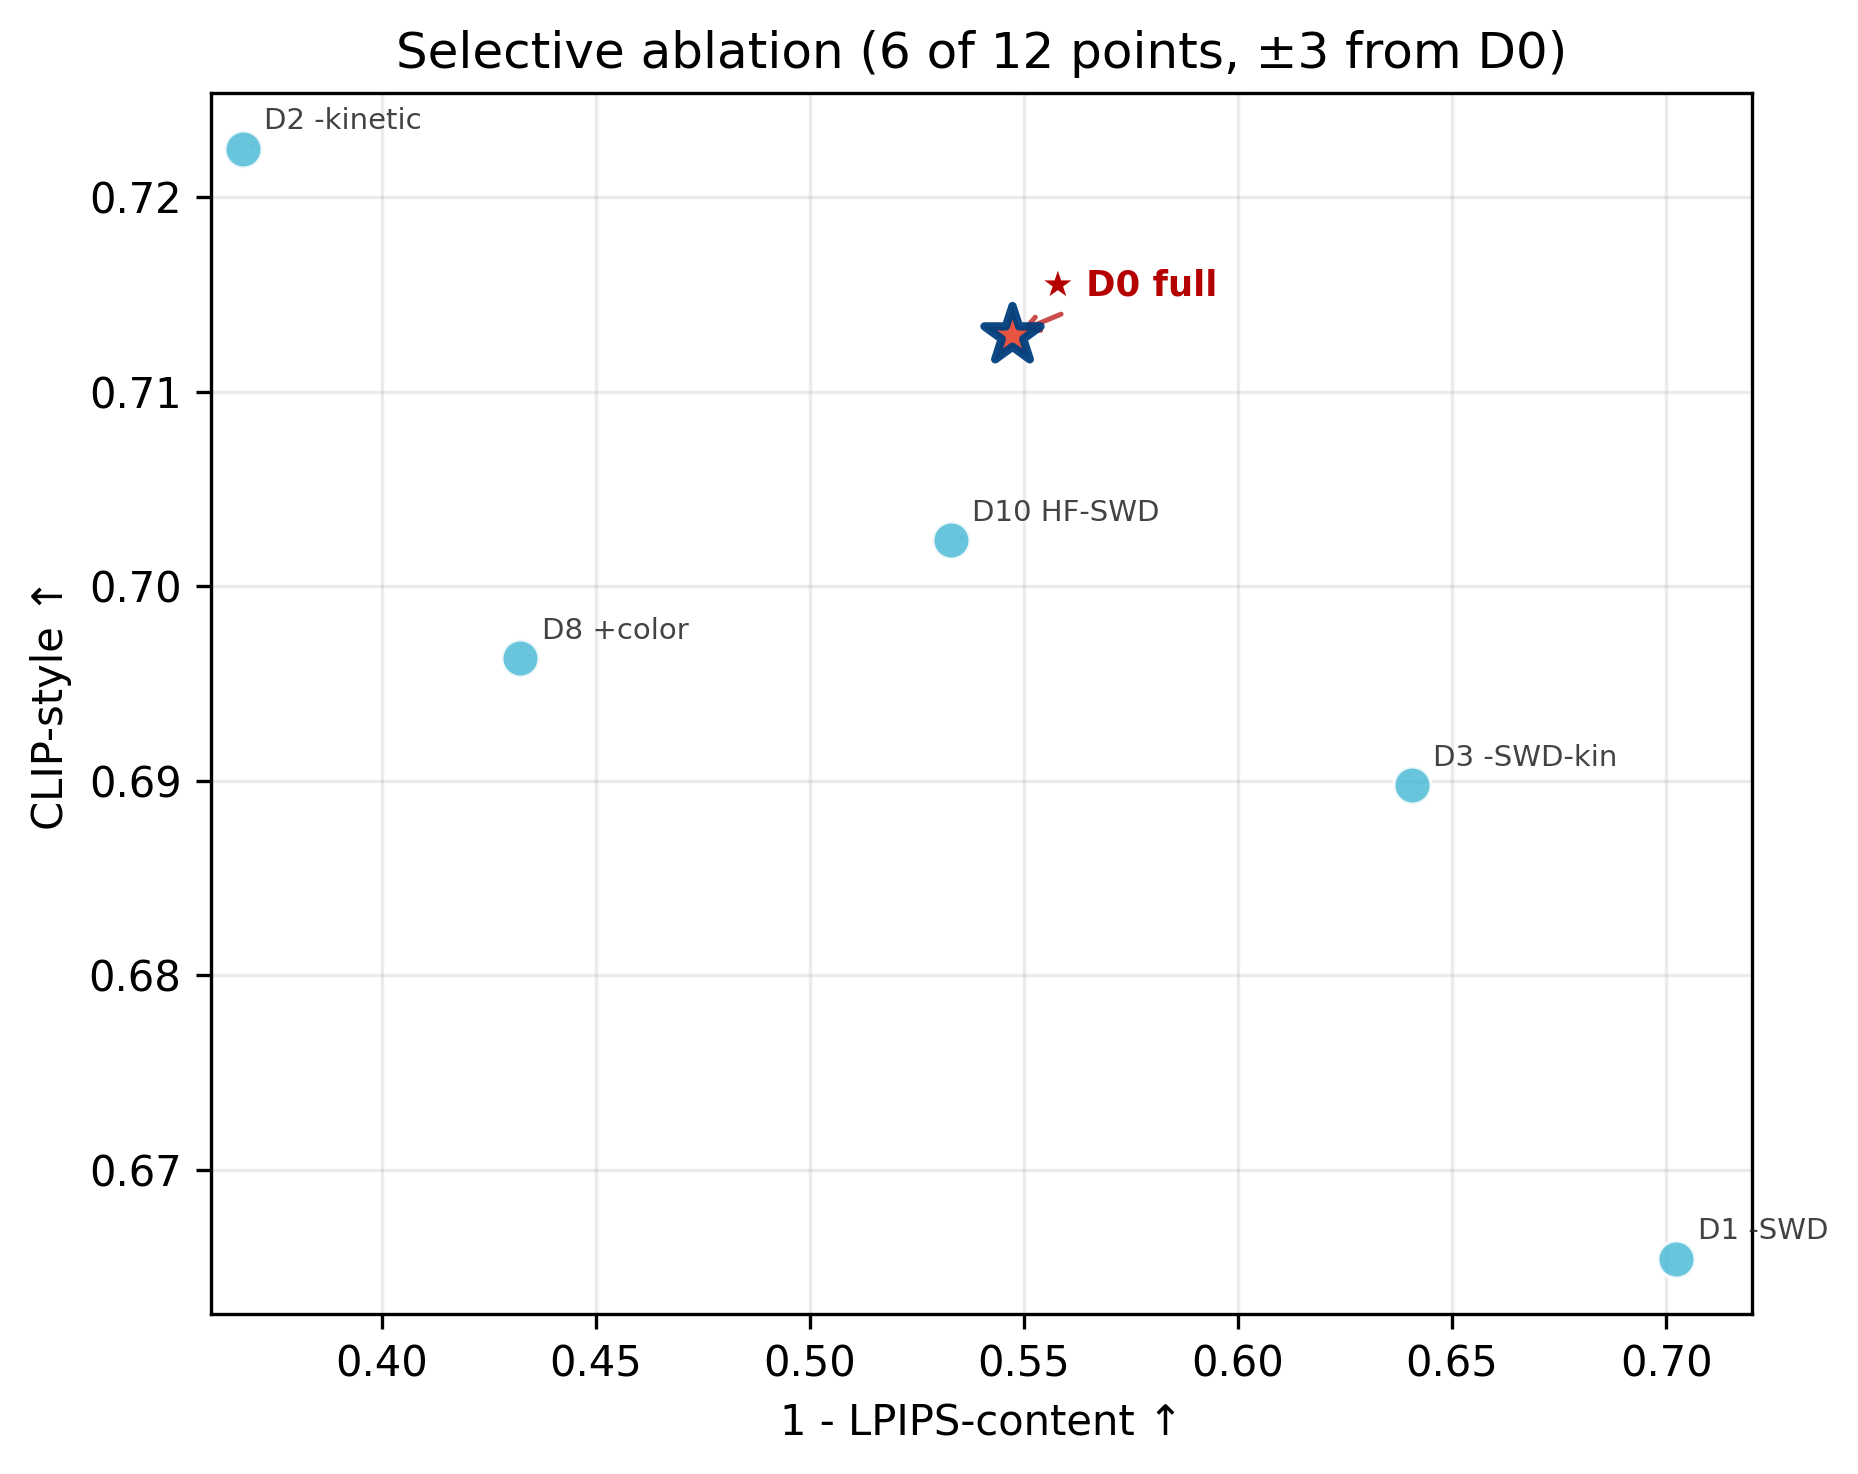
\includegraphics[width=0.82\linewidth]{fig_ablation_pareto.png}
    \caption{Destructive ablations. Removing SA-SWD improves content but weakens style, while removing kinetic regularization increases style at the cost of severe content degradation.}
    \label{fig:ablation}
\end{figure}

\subsection{Weight sweep and theory switches}
The 40-run category-weight sweep trained 20 sampling recipes with $K \in \{1,2\}$ for eight epochs each, evaluating every epoch for 320 total checkpoints. The best EC result was K2 balanced default at epoch 3 with CLIP-style 0.6980, CLIP-content 0.8727, LPIPS 0.3777, and EC 0.4343. The best raw-style result in the sweep was K1 balanced default at epoch 8 with CLIP-style 0.7161, CLIP-content 0.7984, LPIPS 0.4605, and EC 0.3863. The sweep showed that more complex category weighting was not consistently better than balanced sampling.

\begin{figure}[t]
    \centering
    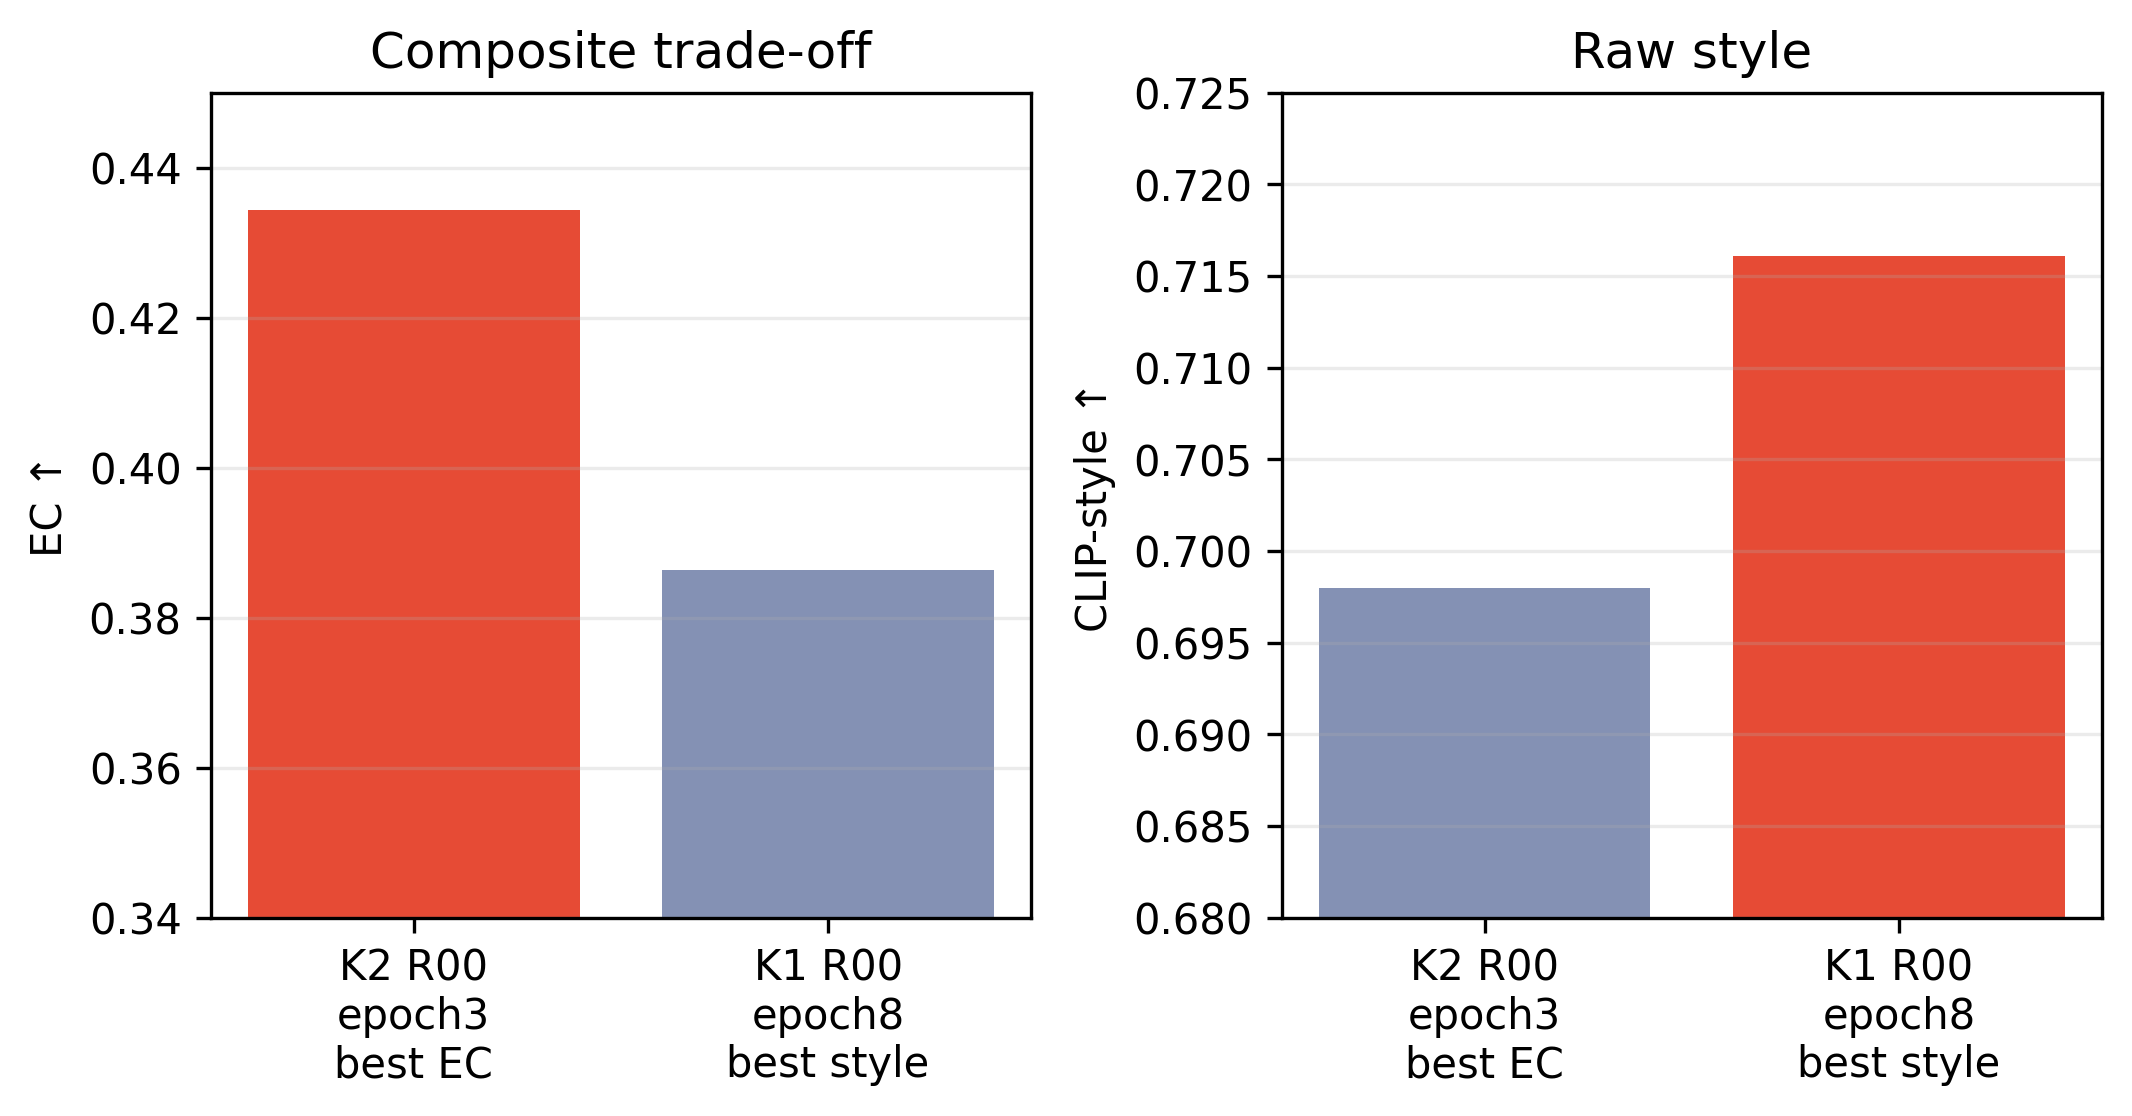
\includegraphics[width=0.86\linewidth]{fig_weight_sweep_summary.png}
    \caption{Summary of the 40-run category-weight sweep. K2 balanced default gives the best EC, whereas K1 balanced default gives the best raw CLIP-style among evaluated checkpoints.}
    \label{fig:sweep}
\end{figure}

\begin{figure}[t]
    \centering
    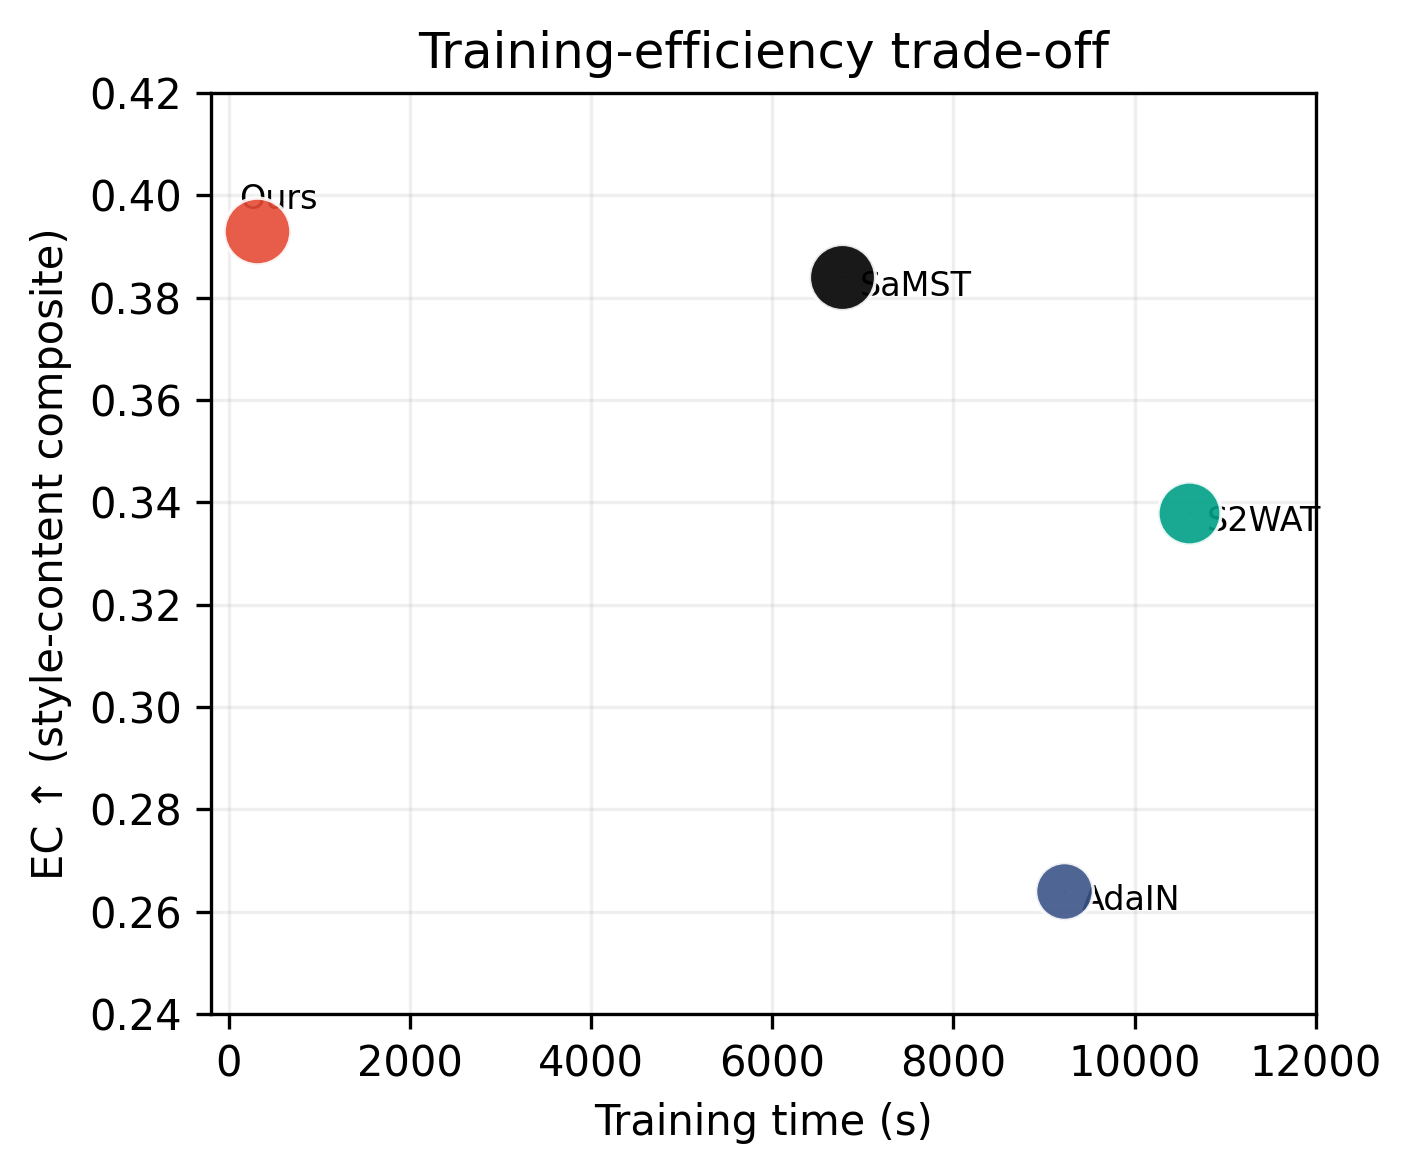
\includegraphics[width=0.82\linewidth]{fig_train_efficiency_pareto.png}
    \caption{Training-efficiency Pareto plot (log scale). Ours achieves the highest EC among compared methods while operating in the lowest training-cost region. Marker size reflects parameter count. Baseline training times follow the extrapolated values ($\dagger$) in Table~\ref{tab:main}.}
    \label{fig:pareto}
\end{figure}

We also evaluated optional theory switches. Sinkhorn-normalized semantic routing and entropy-gated kinetic regularization improved EC/content but reduced raw CLIP-style. The best theory-switch EC was entropy-gated kinetic with weight 5.0 at epoch 1, giving CLIP-style 0.6916, CLIP-content 0.8804, LPIPS 0.3684, and EC 0.4368. Color transport increased raw style slightly but harmed LPIPS and content, and was therefore not selected as the mainline.

\subsection{Step-count and $\lambda$ sensitivity}
The additional step-count sweep evaluates 1, 4, 8, 12, and 16 Euler steps for the selected epoch-7 checkpoint. The main observation is that the quality curve is almost flat over this range. The all-pairs CLIP-style score varies only from 0.7159 to 0.7162, while LPIPS remains tightly concentrated around 0.4514. The photo-to-art operating point is similarly stable: CLIP-style changes only from 0.6712 to 0.6715 and LPIPS remains near 0.4881. This means the 12-step default is not a brittle tuned optimum. In fact, four steps already recover nearly identical quality, while the measured end-to-end strict-750 throughput increases from 8.43 images/s at one step to 9.54 images/s at four steps and remains around 9.34--9.50 images/s for 8--16 steps. The near-flat step curve suggests a stable learned vector field in the selected operating regime, rather than indicating that iterative integration is unnecessary. We therefore keep 12 steps as a conservative default, but the sweep indicates that lower-step deployment is viable when marginal latency reduction matters.

We also scanned a $3 \times 3$ grid over $\lambda_{\mathrm{kin}} \in \{0.5, 1.0, 2.0\}$ and $\lambda_{\mathrm{swd}} \in \{10, 20, 30\}$ for eight epochs each. The resulting surface is smooth and interpretable rather than erratic. Increasing kinetic weight while reducing terminal pressure systematically improves content preservation: at epoch 8, the setting $(2.0, 10)$ yields CLIP-content 0.8734, LPIPS 0.3720, and EC 0.4373, compared with the default $(1.0, 20)$ setting at CLIP-content 0.8124, LPIPS 0.4477, and EC 0.3937. Conversely, weaker kinetic weight or stronger terminal weight pushes the model toward more aggressive but less content-faithful stylization; for example, $(0.5, 30)$ drops CLIP-content to 0.6926 and raises LPIPS to 0.5538. The best transfer-EC checkpoints in this grid occur consistently around epoch 3, again showing that the protocol exposes a broad style-content frontier rather than a single fragile endpoint.

\subsection{Resource use and reproducibility}
End-to-end inference and training times are listed alongside the main metrics in Table~\ref{tab:main}. All timings were measured on an NVIDIA RTX 4070 Laptop GPU (8~GB VRAM) with the same strict-750 protocol. Training times marked $\dagger$ are extrapolated from single-epoch profiling under the same hardware, batch-size policy, and data-loading pipeline; this profiling table is included in the supplementary material. StyleID is training-free by design.

All reported strict-750 evaluations use the same domain protocol and preprocessing pipeline. We also evaluated every epoch in the 40-run sweep, yielding 320 checkpoint evaluations. Final-epoch selection alone can hide style-content trade-offs: K2 balanced default achieved the best EC at epoch 3, whereas K1 balanced default achieved the best raw style at epoch 8. To improve reproducibility, each training run stores the resolved runtime configuration, source-file snapshot, checkpoint, and per-epoch CSV logs. Python, NumPy, PyTorch, and DataLoader worker seeds are fixed per run.



\section{Discussion and Limitations}
LBM prioritizes bounded transport efficiency and artifact-sensitive texture realism in the efficient domain-level regime. The central result is that LBM preserves near-SaMST quality (CLIP-style 0.716 vs.\ 0.719), improves LPIPS and EC, reduces training cost by about $22\times$, and outperforms the heavier S2WAT baseline on core transfer metrics---a favorable efficiency-quality operating point. Importantly, this efficiency gain is not purchased by falling off the quality frontier: it is accompanied by better LPIPS/EC than SaMST and stronger core trade-off metrics than S2WAT.

The current study still has several limitations. First, the style representation is domain-level rather than reference-image-specific; this makes inference efficient but limits the ability to reproduce unique single-image brushstroke patterns or resolve cross-domain prototype conflicts. Second, Euler integration is deliberately simple, so discretization error can accumulate when the latent path is extrapolated to more aggressive settings or higher resolutions. Third, the SWD term uses heuristic multi-scale patch projections rather than an exact transport solver, so the bridge interpretation should remain bounded and practical rather than fully theoretical. Fourth, although the core metrics and efficiency profiling are complete for the compared baselines, the full artifact-diagnostic pack has only been rerun for a subset of methods. Perceptual quality is evaluated via artifact-sensitive diagnostics rather than subjective voting, aligning with our reproducible evaluation protocol. Finally, high-resolution generalization beyond the present 256-based protocol remains under-validated. Code and strict-750 logs will be released upon acceptance to support full reproducibility. Future work should evaluate richer domain prototype priors, controlled integration horizons, higher-resolution extrapolation, and stronger preference-oriented evaluation, including human or rubric-based VLM assessment.

\section{Conclusion}
We presented OT-coupled latent flow matching for efficient domain-level artistic transfer. The method combines three complementary objectives: a flow-matching loss supervises a time-conditioned velocity field along stochastic latent bridges; SA-SWD pulls the integrated endpoint toward the target style distribution along semantic routing axes; and kinetic regularization constrains path displacement to preserve content. Under a strict 750-output evaluation, the resulting 3.9M-parameter model achieves competitive CLIP-style (0.716), the lowest LPIPS among high-style methods (0.451), the best EC score (0.393), and substantially lower training cost than heavier feed-forward baselines---a Pareto-efficient operating point for domain-level artistic transfer.

\FloatBarrier
\bibliography{refs}

\clearpage
\small
\setlength{\itemsep}{1pt}
\setlength{\parskip}{2pt}
\section*{Reproducibility Checklist}
\noindent\textbf{This paper}
\begin{itemize}
\item Includes a conceptual outline and/or pseudocode description of AI methods introduced: \textbf{Yes}.
\item Clearly delineates statements that are opinions, hypothesis, and speculation from objective facts and results: \textbf{Yes}.
\item Provides well marked pedagogical references for less-familiar readers to gain background necessary to replicate the paper: \textbf{Yes}.
\end{itemize}

\noindent\textbf{Does this paper make theoretical contributions?} \textbf{Yes (bounded)}. The paper provides three formal results with proofs and experimental validation (Sec.~\ref{sec:formal}): a path-action decomposition connecting the training kinetic loss to inference-time path energy (Theorem~1), an $O(1/K)$ Euler discretization error bound (Theorem~2), and a Lipschitz-continuity result for the OT assignment map explaining its directional-coherence benefit (Theorem~3). Full proofs are in the supplement. These results constitute a formal justification of the three-part design without claiming equivalence to a full Schr\"odinger Bridge solver.

\noindent\textbf{Does this paper rely on one or more datasets?} \textbf{Yes}.
\begin{itemize}
\item A motivation is given for why the experiments are conducted on the selected datasets: \textbf{Yes}.
\item All novel datasets introduced in this paper are included in a data appendix: \textbf{NA}.
\item All novel datasets introduced in this paper will be made publicly available upon publication of the paper with a license that allows free usage for research purposes: \textbf{NA}.
\item All datasets drawn from the existing literature are accompanied by appropriate citations: \textbf{Yes}.
\item All datasets drawn from the existing literature are publicly available: \textbf{Yes}.
\item All datasets that are not publicly available are described in detail, with explanation why publicly available alternatives are not scientifically satisficing: \textbf{NA}.
\end{itemize}

\noindent\textbf{Does this paper include computational experiments?} \textbf{Yes}.
\begin{itemize}
\item This paper states the number and range of values tried per (hyper-)parameter during development of the paper, along with the criterion used for selecting the final parameter setting: \textbf{Partial}.
\item Any code required for pre-processing data is included in the appendix: \textbf{No}.
\item All source code required for conducting and analyzing the experiments is included in a code appendix: \textbf{No}.
\item All source code required for conducting and analyzing the experiments will be made publicly available upon publication of the paper with a license that allows free usage for research purposes: \textbf{Partial}.
\item All source code implementing new methods have comments detailing the implementation, with references to the paper where each step comes from: \textbf{Partial}.
\item If an algorithm depends on randomness, then the method used for setting seeds is described in a way sufficient to allow replication of results: \textbf{Partial}.
\item This paper specifies the computing infrastructure used for running experiments, including hardware/software details: \textbf{Partial}.
\item This paper formally describes evaluation metrics used and explains the motivation for choosing these metrics: \textbf{Yes}.
\item This paper states the number of algorithm runs used to compute each reported result: \textbf{Yes}.
\item Analysis of experiments goes beyond single-dimensional summaries of performance to include measures of variation, confidence, or other distributional information: \textbf{Yes}.
\item The significance of any improvement or decrease in performance is judged using appropriate statistical tests: \textbf{Yes} (paired bootstrap, 5000 resamples, reported in Sec. Experiments).
\item This paper lists all final (hyper-)parameters used for each model/algorithm in the paper's experiments: \textbf{Partial}.
\end{itemize}

\end{document}



